\section{Materials and Methods}
% This section should be divided by subheadings. Materials and Methods
% should be described with sufficient details to allow others to
% replicate and build on published results. Please note that publication
% of your manuscript implicates that you must make all materials, data,
% and protocols associated with the publication available to
% readers. Please disclose at the submission stage any restrictions on
% the availability of materials or information. New methods and
% protocols should be described in detail while well-established methods
% can be briefly described and appropriately cited.
%
% Research manuscripts reporting large datasets that are deposited in a
% publicly available database should specify where the data have been
% deposited and provide the relevant accession numbers. If the accession
% numbers have not yet been obtained at the time of submission, please
% state that they will be provided during review. They must be provided
% prior to publication.

This section covers the materials and methods for ROSMOD and the AGSE,
both what was used in the competition (2014-2015) as well as the
current state of each.

\subsection{Competition AGSE}

The version of the AGSE software and hardware designs that were used
in the 2014-2015 NASA SLI competition can be found open-sourced
online\cite{AGSE2015}. The current version of the AGSE code and
hardware designs has been moved and can be found in the Vanderbilt
Aerospace Design Lab's AGSE repository\cite{AGSE}.

\subsubsection{Kinematics}
%describe the joint structure of the robot, detail the coordinate system, etc.

The AGSE is a 4-DOF robot utilizing a revolute base joint to rotate
the robot body, two prismatic joints to move vertically and
horizontally, and a final revolute joint providing an orienting wrist
for the end effector. A wireframe and workspace rendering of the AGSE
can be seen in Figure \ref{fig:Render}.


\begin{figure}[h]
	\centering
        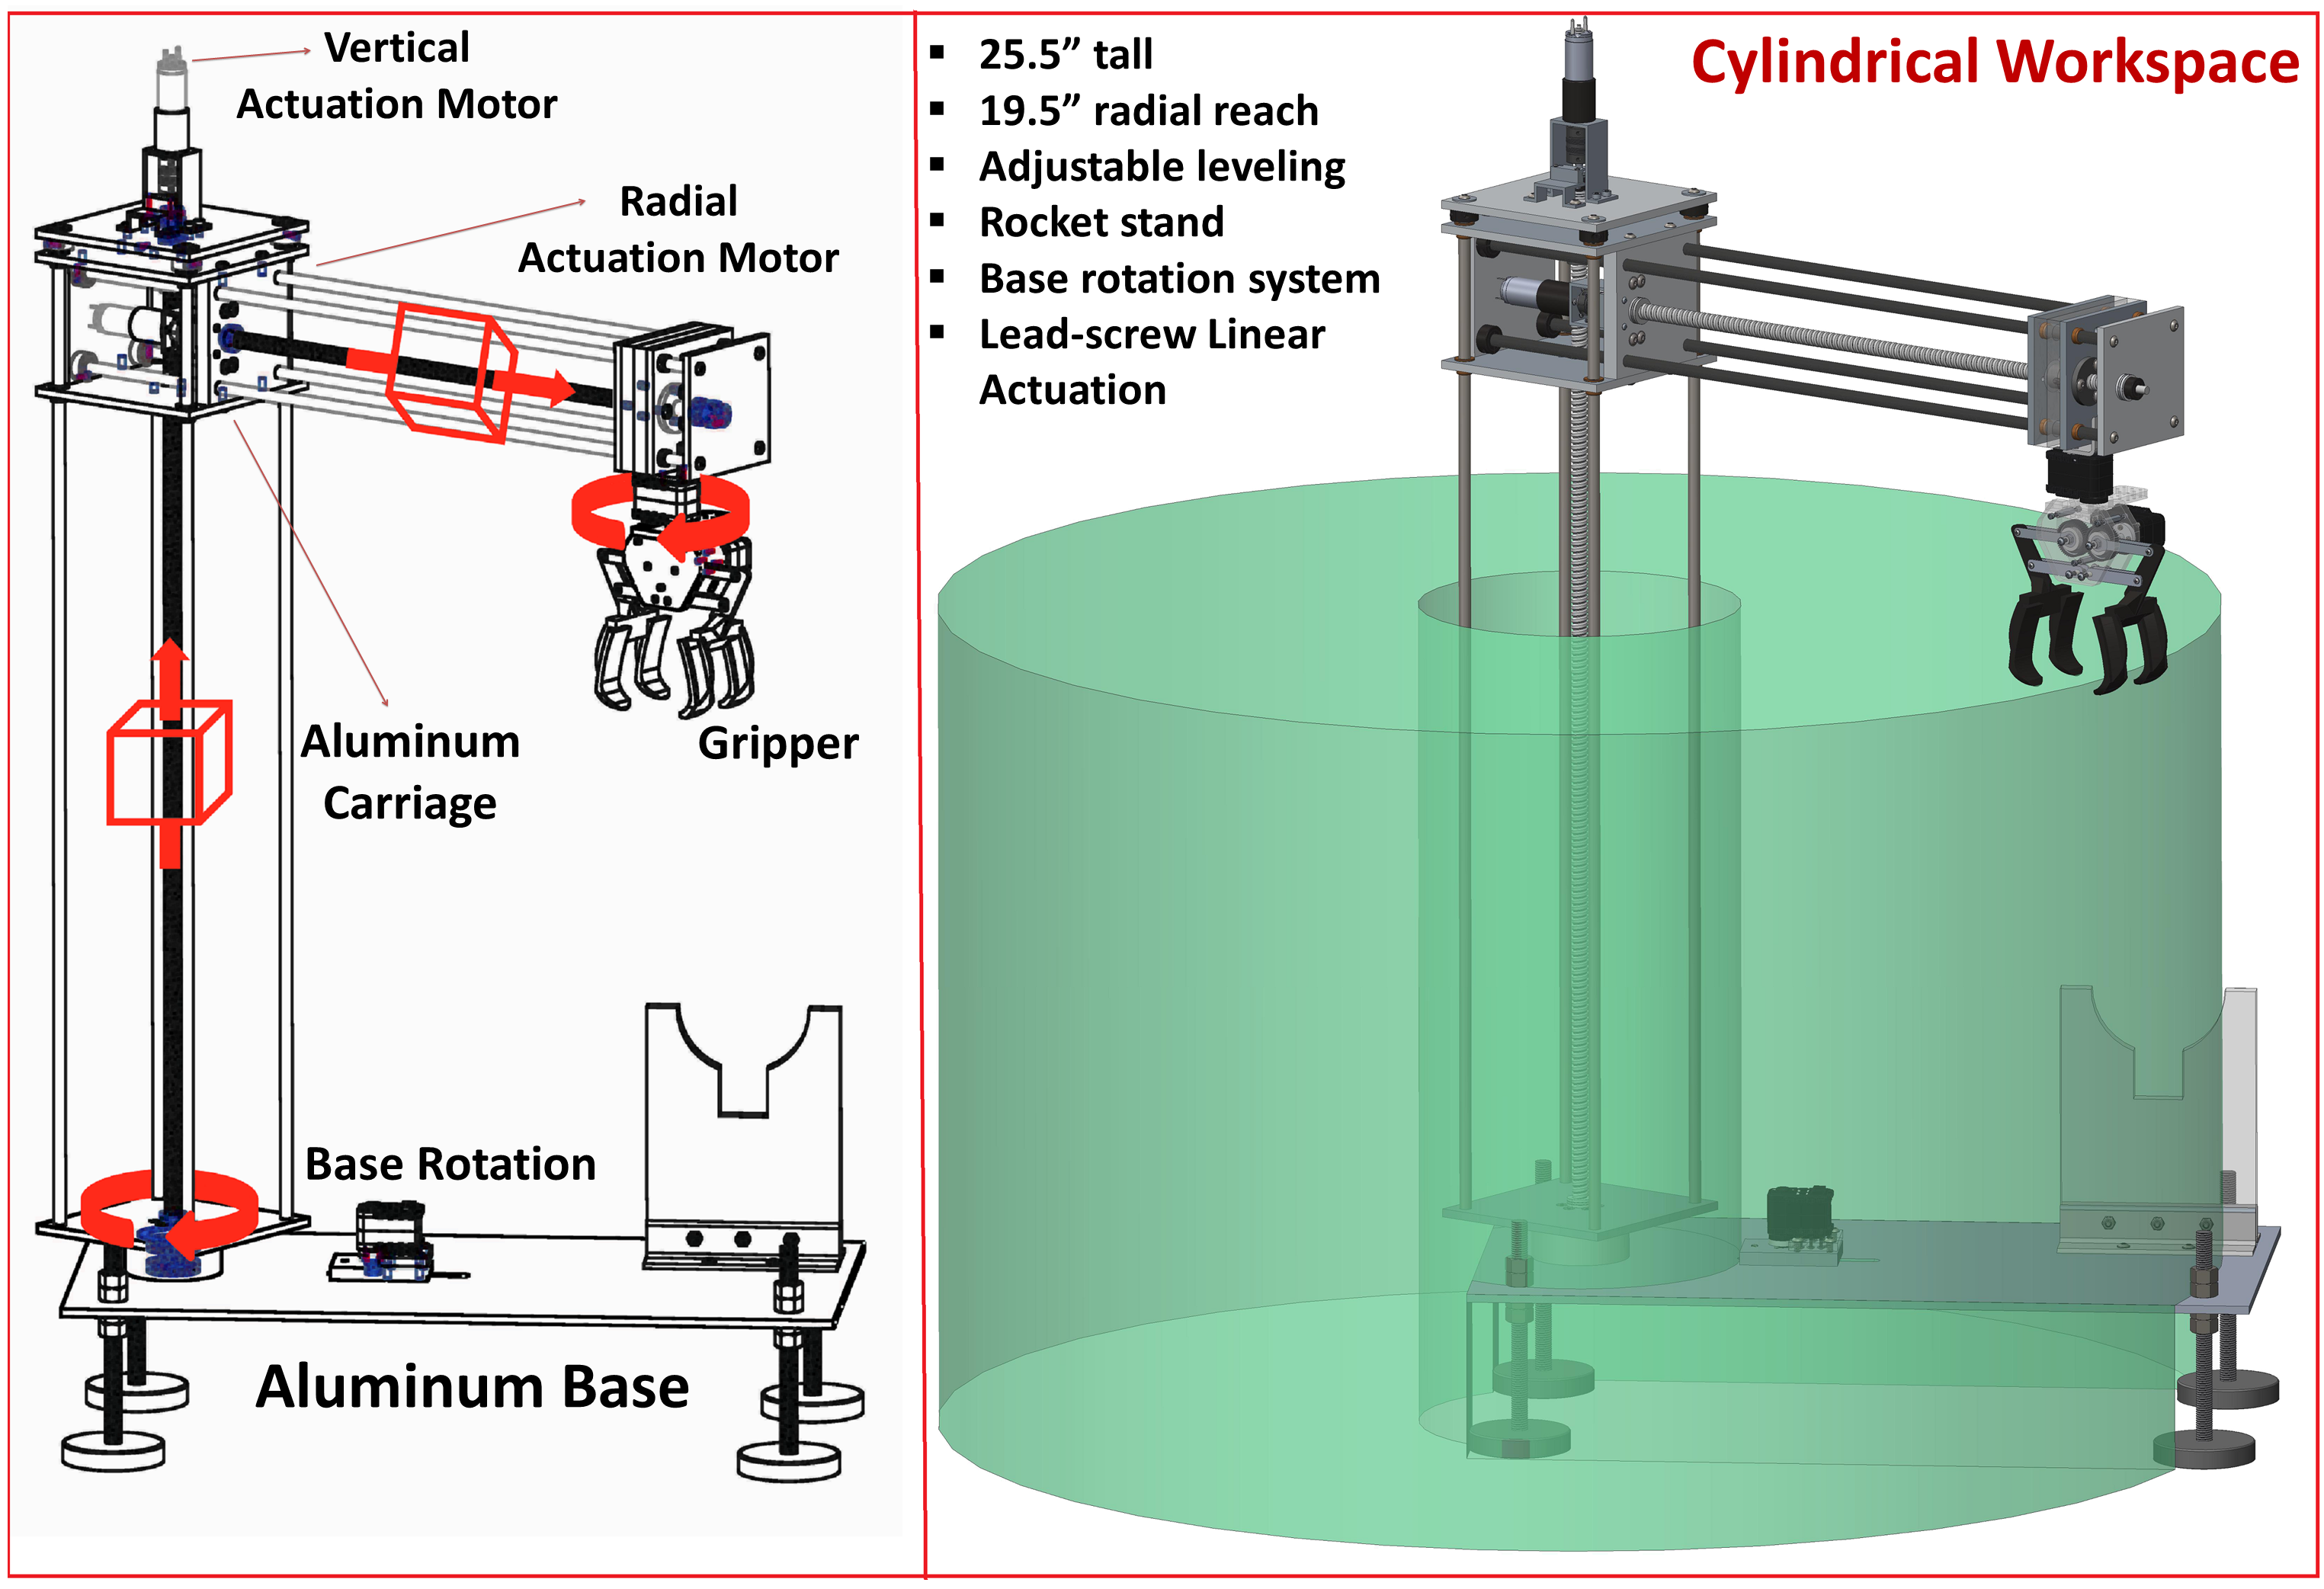
\includegraphics[width=\textwidth]{./Figures/AGSE_Mechanical_Design_Figure.png}
	\caption{AGSE Mechanical Design}
	\label{fig:Render}
\end{figure}

%description of coordinate system
By design, the single revolute and two prismatic joints of the AGSE
provide the basis for a cylindrical coordinate system and workspace,
reducing the implementation of both forward and reverse kinematics to
a trivial exercise of mapping joint position to the corresponding
coordinate in the workspace.

$$
\begin{bmatrix}
	\boldsymbol{\theta}_{workspace}\\\mathbf{r}_{workspace}\\\mathbf{z}_{workspace}
\end{bmatrix}=
\begin{bmatrix}
	\boldsymbol{\theta}_{rev}\\\mathbf{r}_{pris}\\\mathbf{z}_{pris}
\end{bmatrix}
$$
%?equations of end-effector position based on joint posiiton?

\subsubsection{Structure}
%describe the physical structure of the base, each joint starting at the base, mounting hardware for electronics

The AGSE base is comprised of a machined sheet of aluminum upon which
leveling legs are mounted to easily account for uneven surfaces.
Protruding from the base is the revolute joint, a machined spindle
centered within ball bearing cup. Extending upwards along this
rotational axis is the vertial join, a lead screw and guide rod
assembly driving an aluminum carriage. A similar lead screw-carriage
assembly extends from the side of the vertical carriage to provide
motion within the horizontal plane. A mounting point for both the
gripper and camera hangs from this horizontal carriage.

Underneath the base is a platform for mounting batteries, power
regulation and protection circuitry, and on-board computer systems.  At
the top of the vertical assembly is a mounting point for the actuator
control electronics.


\subsubsection{Actuation and Sensing}
%detail the actuators used for each joint and all sensors utilized

A Dynamixel MX-28T servo is mounted to the revolute joint's spindle to
provide rotational movement. Two additional Dynamixel AX-12 servos are used
to orient and actuate the gripper. The two lead screw assemblies are
driven using 12 V Faulhaber motors mounted directly to the lead
screws.

The AGSE guides the end effector motion using the limit switch-encoder
combo on its linear actuators, the built in positional feedback from
the servo motors, and the optical feedback provided by a camera
mounted above the end effector (allowing the AGSE to recognize objects
within the reachable area underneath the gripper phalanges).  Limit
switches are mounted at the minimum and maximum of each lead screw
assembly's range of movement, providing hard stops to motor actuation.
Quadrature encoders are then used within this range of motion to
monitor the position of the vertical and horizontal carriages. The
Dynamixel servos controlling the revolute joint and gripper provide
position and speed feedback, as well as PID tuning to allow for quick
and responsive control.

\subsubsection{Power System}
%What powers it: Originally 2 12v batteries, now using power supply
%On/Off with relay
%Power Protection: Originally none, now have a fuse board
%

The power from the AGSE comes from two 12V 12Ah lead-acid batteries in
series, which provide input power to a 12V power regulator.  The 12V
output from the power regulator passes through a relay which is
controlled using a key-switch on the User Interface Panel (UIP).  From
the relay the 12V runs in parallel to the NVIDIA Jetson TK1, the Motor
Control Cape on the Motor Control BeagleBoneBlack, the User Interface
Panel power control cape (a stripped down version of the Motor Control
Cape with the H-Bridges and other motor related electronics not
populated), and finally to the ethernet switch which provides a
closed, hard-wired LAN for communications between the boards.

On the Motor Control Board, the 12V input drives 1) the cape's 5V
regulator which provides power to the BeagleBone Black and the
encoders, 2) the 12V Dynamixel servo motors, and 3) the H-Bridges for
the two 12V linear actuators.

On the UIP, the 12V simply powers the 5V regulator which provides
power to the BeagleBone Black, the touchscreen LCD, and the display
LEDs.

\subsubsection{Control}
%Touch on these topics: Low-Level Motor Control, High-Level control  (Introduce image processing and path planning), feedback processing

The payload bay and nose section of the rocket rests on the base of
the AGSE. This payload bay is motor-controlled by the high-level
controller. When the AGSE starts up, the payload bay's on-board Arduino motor controller is
commanded to open the nosecone. Once open, the AGSE performs an initialization
routine. This routine includes movement of the vertical and radial
actuators to a safe height and a retracted state. Then, the AGSE
rotates on its base to a servo angle of zero degrees. Once this
routine is complete, the robots begins searching for the sample. The
camera used for this purpose is a 1920x1080 wide resolution feed; one
that enables the robot to sweep wider distances when searching for the
sample and increases the step size of the search i.e. the search steps
up by 20 degree increments while searching for the sample.

\begin{figure}[h]
	\centering
	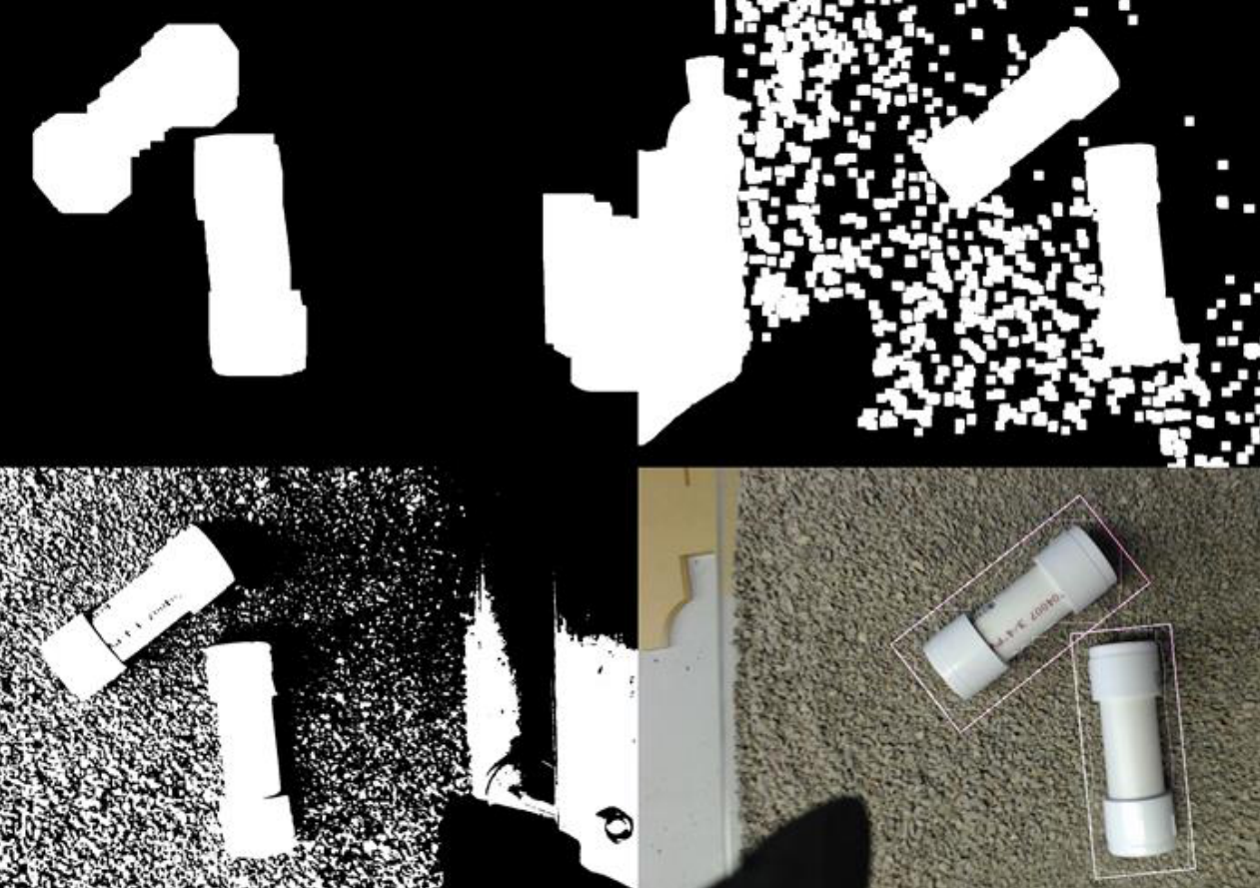
\includegraphics[width=0.75\textwidth]{Figures/Sample_Image_Processing_2.png}
	\caption{AGSE Sample Detection - Periodic Image Processing}
	\label{fig:Sample_Image_Processing_2}
\end{figure}

Periodic sample detection performed by the AGSE uses OpenCV-based
image processing algorithms to identify and track the sample in
real-time. An Image Processor component periodically fetches the
latest feed from the mounted camera and performs a series of filtering
tasks. Each \emph{RGB} (Red-green-blue) image frame is converted to
both \emph{HSV} (Hue-Saturation-Value) and \emph{Grayscale} image
frames. After applying thresholds, filters, erosion and dilation
methods, the target sample is extracted from the webcam feed. Once the
target sample is detected, as shown in Figure
\ref{fig:Sample_Image_Processing_2}, we draw contours around the
object and identify its relative position and orientation.

Once the sample is detected, the AGSE records the position and
orientation of this sample and begins searching for the payload
bay. The payload bay is detected using marker detection methods. Coded
markers are stuck on the payload bay to detect the angle at which the
sample needs to be dropped into the bay. As shown in Figure
\ref{fig:Payloadbay_Detection}, by processing the input camera feed,
the two markers on the bay are detected and the angle of drop is
calculated.

\begin{figure}[h]
	\centering
	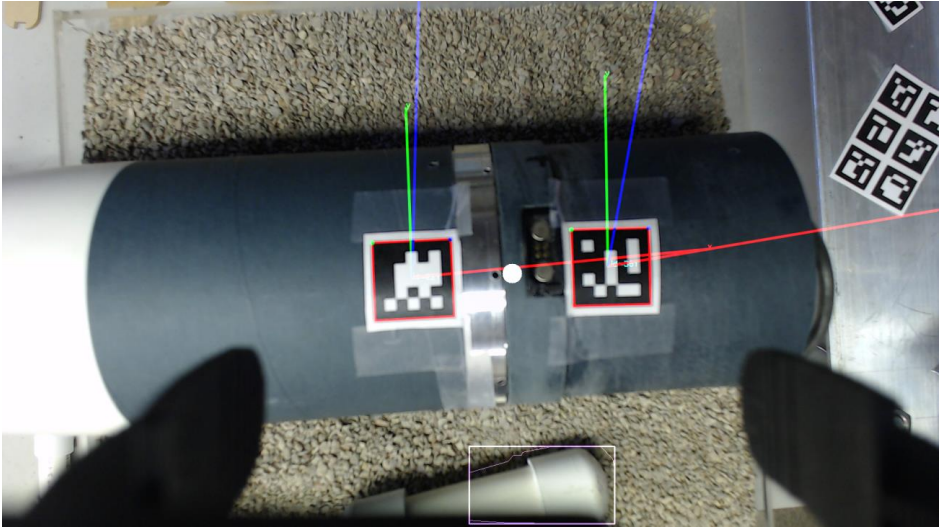
\includegraphics[width=0.75\textwidth]{Figures/Payloadbay_Detection.png}
	\caption{AGSE Payload Bay Detection}
	\label{fig:Payloadbay_Detection}
\end{figure}

Once the sample and payload bay are fully detected, the AGSE performs
a simple pickup-drop transition where it rotates to the position of
the sample, grabs the sample, rotates to the position of the payload
bay and drops the sample in the bay. The arm control logic also sends
a \emph{"Close Payload Bay"} command that actuates the payload motor
and closes the nosecone, effectively completing the sample retrieval
process.

\subsubsection{Communication}
%How do the components communicate? Servos daisychained and identified by device ID and controled via modified dynamixel library, BBB, Jetson, and UIP connected to network with static IPs, etc.

The AGSE communicates between its various subsystems using a few
different protocols.  At the high level, the different control boards
of the AGSE communicate using ROS over a wired ethernet LAN.  On the
motor control board, the servo motors are directly connected to a 3.3V
serial port on the GPIO pins of the BeagleBone Black.  Because the
servo motors communicate at 5V using a 1-wire communications line, the
communications transmitted to the servos from the BeagleBone Black
passes through a buffer implemented with NPN transistors.  Because the
servos can be daisy-chained, only one connection is made to the Motor
Control Cape and each servo is connected in series through the
previous servo.  This daisy-chaining greatly simplifies the wire
routing and increases the modularity and maintainability of the AGSE
motor hardware.  Finally, the NVIDIA Jetson communicates to the
Payload Bay Arduino to open and close through its own USB port acting
as a virtual serial port.  This serial connection is implemented as a
quick-disconnect USB cable connected to a port on the surface of the
rocket.

\subsection{AGSE Changes Since the Competition}

Post competition, minor mechanical and electrical improvements were made to the AGSE.  A new mounting bracket was machined to replace the temporary mounting of the Dynamixel MX-28T that occurred the day of the competition. A new undercarriage made of extruded 20mmx20mm aluminum was fabricated to house the on-board power circuitry and embedded systems.  Additionally, new power protection circuitry was made in the form of fuse boards and a dedicated emergency stop button in lieu of the key switch in the UIP.

\subsection{Competition ROSMOD}

ROSMOD exists as two separate code-bases: 1) the ROSMOD component
model implementation, which enables the configuration of the component
operation queue to support different scheduling schemes and
priorities/deadlines for operations, and 2) the ROSMOD graphical
modeling, generation, and deployment tool suite.  These two code-bases
are referred to as ROSMOD-COM and ROSMOD-GUI, respectively.  All
ROSMOD related code (old and new) can be found open-sourced online in
the ROSMOD Github organization\cite{ROSMOD_ORG}.

ROSMOD-COM is a package which extends the functionality of the
\emph{ROS Callback Queue} into which timer, subscriber and service
operations are placed.  To enable the addition of scheduling,
priority, and deadline attributes to operations in the queue, all the
relevant objects were modified, e.g. Timer, Subscriber, etc.
Additionally, the queue was extended to support priority insertion of
operations based on their deadline (EDF scheduling) and priority
(PFIFO).  By using the relevant classes and methods from ROSMOD-COM,
ROSMOD components can ensure the proper scheduling of their
operations.

The version of ROSMOD that was used in the competition can also be
found open-sourced online\cite{ROSMOD}, as the \emph{v0.3-beta}
release.  Note that the version of the ROSMOD-GUI that was used is
under the \emph{gui} folder and is a Python-based program for which
the relevant dependencies must be installed following the
\emph{README}.  This is one of the primary problems with this version. Firstly, ROSMOD requires Linux and the Python programming language and a long list of dependencies. Also, this version, as used in the competition was primarily used for code generation and compilation. The deployment framework had several shortcomings, primarily due to the metamodeling language at the time. Many of these shortcomings have now been addressed e.g. the concept of an experiment, a much improved network model etc. 

\subsection{ROSMOD Changes Since the Competition}
The current version of ROSMOD is split into two
separate repositories under the ROSMOD organization: the new version
of the GUI\cite{ROSMOD_WEBGME}, and the current version of
ROSMOD-COM\cite{ROSMOD}.

ROSMOD-COM has been updated to be a standalone ROS package so that it
no longer has to be compiled inside ROS' source tree.  Upon installing
ROSMOD-COM, the scheduling schemes and associated configuration and
classes become available for use in all packages.

ROSMOD-GUI has been transformed into a more fully integrated
development environment which is now platform independent as it runs
within the browser.  The server runs within a Linux environment and
can be locally deployed on a laptop or virtual machine, or on a real
server.  The change to this new infrastructure was enabled by the
switch to using WebGME\cite{maroti2014next} as the backend for the modeling and
server execution.  This change also enables collaborative
simulataneous model creation and editing between multiple users, with
built-in git-sytle versioning, branching, and merging.

Despite the increase in backend complexity and number of features of
ROSMOD, the use of ROSMOD and the installation of the backend has
become far simpler and completely automated by widely-used packaging
tools.  The repository has installation instructions and users guides.
